% vim: set spell : spelllang=en_gb
\title{\bf Dynamic priority broadcasting channels:\\
	a multi-objective planning problem}
\author{Chiel Kooijman - 5743028\\University of Amsterdam}
\documentclass{article}
\usepackage{graphicx,amsmath}
\usepackage[round]{natbib}
\usepackage{multicol}
\usepackage{caption}
\usepackage{subcaption}
\usepackage{geometry}
\usepackage{algorithm}
\usepackage{algpseudocode}
\usepackage{comment}
\usepackage{amssymb}
\def\keywords{\vspace{.5em}
	{\textbf{Keywords}:\,\relax
}}
\def\endkeywords{\par}
\newenvironment{tablehere}
{\def\@captype{table}}
{}

\newenvironment{figurehere}
{\def\@captype{figure}}
{}

\date{}
\setlength{\textwidth}{6.5in}
\setlength{\oddsidemargin}{0in}
\setlength{\evensidemargin}{0in}
\thispagestyle{empty}
\begin{document}
	\setlength{\footskip}{3cm}
	\maketitle

	\begin{abstract}
		This article explores the broadcasting channel problem, focusing on
		dynamic priority planning. We will show that using the Pareto-optimal set
		of solutions significantly reduces the set size and computation time, but
		that it is still infeasible. We propose a method for reducing computation
		time of generating the Pareto-optimal set and show that pruning is
		necessary.
	\end{abstract}
	\begin{keywords}
		Dynamic Programming, MDP, Markov Decision Process, Multi-objective,
		Planning, Broadcasting Channel, Dynamic Priority, Pareto-optimal set
	\end{keywords}

	%\tableofcontents
	%\clearpage
	\begin{multicols}{2}

	\section{Introduction}
	\label{sec:introduction}
	In this research we extend the broadcasting channel problem as defined by
	\citet{ooi1996decentralized}, in order to account for situations in which
	multiple objectives are important, such as workload distribution in a data
	environment, distribution of traffic, or prioritisation of more important
	messages, in addition to throughput.
	In section \ref{sec:problem_definition} we redefine the problem to account
	for these considerations. Section \ref{sec:approach} covers the methods used
	to meet these requirements, and some implementation specifics. The results
	are described in section \ref{sec:results}, and section \ref{sec:discussion}
	proposes an algorithm that exploits the properties of the data to reduce the
	time complexity of calculating the Pareto-optimal set.
	% section introduction (end)

	\section{Problem definition}
	\label{sec:problem_definition}
	Multiple agents broadcast messages over a single channel, but only one
	message can be sent at any time, otherwise conflicts will arise and no
	message will come through. After a message is sent, the agents will know
	whether a message was sent, a conflict has arisen, or no message was sent.
	Agents have a single buffer that may contain a message. A visualisation of a
	two-agent setup is shown in figure \ref{fig:agents_ee}.

	\vspace{0.5cm}
	\begin{figurehere}
		\centering
		\includegraphics[scale=0.3]{images/agents_ee-crop}
		\captionof{figure}{A setup with two agents}
	   \label{fig:agents_ee}
	\end{figurehere}
	\vspace{0.5cm}

	At any concrete time-step an agent $i$ with an empty buffer may get a new
	message with probability $p_i(s' |s, \vec{a})$.
	The problem of optimising throughput has been solved for POMDPs
	\citep{ooi1996decentralized, hansen2004dynamic}, but in this case we would
	also like to take into account other goals such as avoiding dominance of a
	single agent over the channel or guaranteeing a certain throughput for an
	important agent.

	\citet{hansen2004dynamic} have provided a solution with dynamic programming.
	This method will be extended so that for any weight vector $\vec{w}$ it will
	return the optimal Pareto-optimal set of solutions $\vec{w} \cdot
	\vec{V}^\pi$ \citep{vamplew2011empirical}, in a reward representation that
	can dynamically adapt priorities by changing the weights
	\citep{barrett2008learning,natarajan2005dynamic}.

	\subsection{Relevance}
	\label{sub:relevance}
	Real-world situations that may benefit from this research may include
	operating system schedulers, collaborative multi-agent communication, and
	home networks.

	For instance the Completely Fair Scheduler (CFS) that is used in the Linux
	kernel (as of the 2.6.23 release), prioritises tasks that use less time.
	This may not be the ideal solution, as tasks that only need to be performed
	on a slow interval are often not of a high priority. Tasks such as user
	interaction may require a fair amount of computation time, but this should
	not reduce its precedence with regard to background tasks, as the user will
	notice lags former more than in the latter.

	An example of a collaborative system are rescue robots that work together on
	mapping an environment in order to effectively find and rescue victims from
	sites such as collapsed buildings or mines. Sharing all information as it is
	acquired could be too heavy a burden on the network, and dynamic
	prioritisation could be used to make the most efficient use of the available
	bandwidth. Priority of the agent would be based on measures such as expected
	information gain.

	A home network could include telephones, televisions, and personal
	computers. Although we may want to prioritise the telephones and television
	to guarantee continuity, we would also like to reduce lag in tasks that are
	requested by the user such as loading a website. Telephone and television
	prefer a specific continuous amount of throughput, but after some value do
	not benefit much more, whereas other tasks may always benefit from more
	throughput, such as downloading large files. When an alarm call is made, we
	would like to guarantee the quality of the line before all else, but not
	drop other tasks if it can be avoided. Many requirements may change over
	time as devices phone calls are ended or personal computers are connected to
	the network.
	% subsection relevance (end)
	% section problem_definition (end)

	\section{Approach}
	\label{sec:approach}

		\subsection{Reward Representation}
		\label{sub:reward_representation}
		There are several ways to represent throughput and dominance in a vector.
		One approach is to have a two-dimensional vector $\vec{r}$ that contains
		the total throughput and some measure of dominance, for instance entropy
		or variance. An advantage of this approach is that the size of the reward
		vector is independent of the number of agents.

		Another way is to represent the vector as an $n$-dimensional vector:
		$$\vec{r} = \begin{bmatrix}
			t_1\\
			\vdots\\
			t_n\\
		\end{bmatrix}$$
		where $n$ is the number of agents, and each value represents the
		throughput of the corresponding agent. An advantage is that the vector
		contains more information than in the aforementioned representation,
		which allows us to use different measures of optimality, but
		there are many more states when the number of agents increases. It does
		however allow for prioritising messages, and when we choose not to
		prioritise, the number of states can be greatly reduced, because every
		vector is equal to all of its permutations (provided we reorder the state
		vector and the reward vector in the same way).
		For example in a two-agent system, a state with a reward vector $\vec{r}$
		and function parameter $\vec{\theta}$
		vectors
		$$ f_{\vec{\theta}}(\vec{r})~\textrm{with}~\vec{r} = \begin{bmatrix}
			7\\
			3\\
		\end{bmatrix},~
		\vec{\theta} = \begin{bmatrix}
			w_1\\
			w_2\\
		\end{bmatrix}$$
		the value is equal to that of
		$$ f_{\vec{\theta}}(\vec{r})~\textrm{with}~\vec{r} = \begin{bmatrix}
			3\\
			7\\
		\end{bmatrix},~
		\vec{\theta} = \begin{bmatrix}
			w_2\\
			w_1\\
		\end{bmatrix}$$
		because all agents are equal and connected to the network in the same
		way.
		For these reasons the second representation was chosen.

		This method can also be extended to a multi-channel set-up: Where we
		would reward only one agent, and only when it was the only agent to send a
		message in the single-channel set-up, we can reward any number of agents
		that sent a message, if there were no more messages sent than the number
		of channels.
		% subsection reward_representation (end)

		\subsection{State Representation}
		\label{sub:state_representation}
		The Bellman equation \ref{eq:bellman} describes the value $V$ of a state
		$s$ given policy $\pi$. It is defined by the return $R$ that is obtained in
		state $s$, plus the expected return in the following states $s'$given the
		policy. Discount value $\gamma$ is a value in $[0, 1)$, and defines the
		weight of future rewards. Low values can be seen as making the agent
		impatient, because a states value is mostly defined by expected return in
		the near future.
		\begin{equation}
		\displaystyle
		V(s)^\pi = R(s) + \gamma\sum_{s'} P(s'|s, \pi(s)) V^\pi(s')
		\label{eq:bellman}
		\end{equation}

		In a system with an event horizon we can represent a state as a vector of
		booleans, that represents for each agent whether it has a message to send
		or not. Furthermore, discounting is unnecessary when calculating state
		values, whereas in a system without a horizon discounting the reward is
		necessary to make the values converge. With Dynamic Programming (DP) we
		can calculate the optimal policy. Values for the states can be redefined
		as shown in equation \ref{eq:bellman_dp}.

		\begin{equation}
		\displaystyle
		V(s)^* = R(s) + \max_a \sum_{s'} P(s'|s, a) V^*(s')
		\label{eq:bellman_dp}
		\end{equation}

		In our case it may be more useful to represent values of state-action
		pairs, as the immediate return $R$ is dependent on the action given the
		state. Equation \ref{eq:bellman_q} shows how this value $Q$ can be
		calculated.
		\begin{equation}
		\displaystyle
		Q(s, a)^* = \sum_{s'} P(s'|s, a) \left(R(s, a) + \max_{a'} Q^*(s', a')\right)
		\label{eq:bellman_q}
		\end{equation}

		As the $\max$-operator is not defined for vectors, the output consists of
		a set of vectors instead of a scalar. To reduce the size of this set, we
		only use the subset of Pareto-optimal values, which contains all optimal
		values for any definition of optimality we would choose in this task.
		A vector belongs in a Pareto-optimal set if there are no other vectors
		that are higher or equal in all dimensions.

		Equation \ref{eq:pareto} shows the definition for the Pareto-optimal set.
		\begin{equation}
			\label{eq:pareto}
			\Big\{ V\, \Big| \, \forall V'[ V \neq V' \land \exists n [V_n > V'_n]] \Big\}
		\end{equation}
		An example of a Pareto-optimal set for a two-dimensional system is shown in
		figure \ref{fig:pareto}.

		\vspace{0.5cm}
		\begin{figurehere}
			\centering
			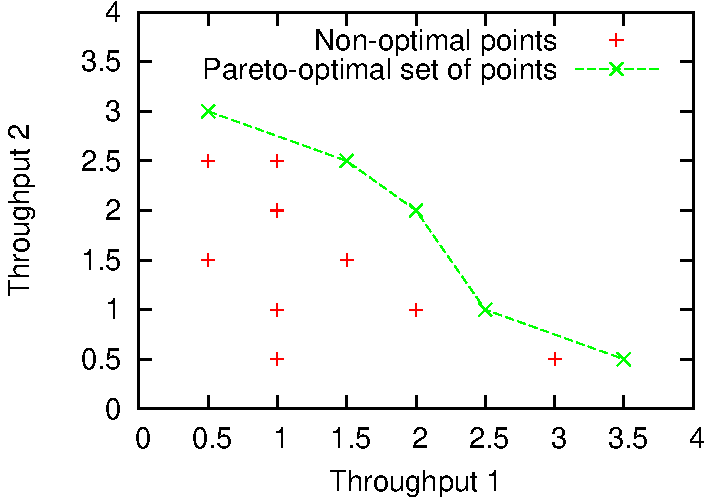
\includegraphics[width=\columnwidth]{images/pareto}
			\captionof{figure}{Pareto-optimal set in a two-dimensional system}
			\label{fig:pareto}
		\end{figurehere}
		\vspace{0.5cm}

		The number of different possible states is $2^n$ where $n$ is the number
		of agents. In the fully observable system there are up to $n+1$ possible
		actions: any one agent can send a message or none at all. In a system
		where agents are unable to observe the states of other agents there are
		up to $2^n$ possible actions as any combination of agents can send a
		message.
		% subsection state_representation (end)

		\clearpage
		\subsection{Implementation}
		\label{sub:implementation}
		The planning algorithm was implemented in C++, as it allows for low-level
		optimisations as well as object-oriented programming and generic
		programming, and a wide array of libraries such as The Standard Template
		Library (STL), are available.
		The goal of the algorithm is to compute the values for every action in
		every state of every time, given that it will follow an optimal policy.

		States and actions are represented as integers, which can be seen as
		arrays of booleans. For example, binary $0100$ represents the
		\emph{state} where only the third agent has a message, or the
		\emph{action} where only the third agent sends a message, dependent on
		context. This representation is used to improve performance.

		Algorithm \ref{alg:main} shows the main loop of the algorithm. Starting
		from the last time-step (at $t=0$) we calculate the reward of all
		possible actions.
		While the value at $t=0$ is only dependent on direct reward, for the
		other time-steps it is the sum of the direct reward for taking the action
		and the weighted average of the values of the possible transition states
		(multiplied with the probability of reaching that state given the
		action). On line \ref{alg:main:increment} the action is converted to an
		index (i.e. $0100$ to 3), and 1 (the direct reward) is added to the
		vectors in that dimension.

		\end{multicols}
		\begin{algorithm}[h]
			\captionof{algorithm}{Main Loop}
			\begin{algorithmic}[1]
				\Procedure{main}{$\mathit{n\_agents}, \mathit{time}, \mathit{p\_msg}[]$}
				\State $\mathit{n\_states} \gets \Call{pow}{2, \mathit{n\_agents}}$
				\State {$Q[\mathit{max\_t}][\mathit{n\_states}]$} \Comment{Initialise Q}
				\For {$t \gets 0, \mathit{time}$}
				\For {$s \gets 0, \mathit{n\_states}$}
				\State $\mathit{actions} \gets \Call{get\_actions}{s, \mathit{n\_agents}}$
				\ForAll {$a \in \mathit{actions}$}
				\State $\mathit{rewards}[] \gets \Call{trans\_rewards}{a, s, \mathit{n\_states}, \mathit{p\_msg}}$
				\Comment{States multiplied with probabilities}
				\State $\mathit{new\_rewards} = \Call{add\_sets}{\mathit{rewards}}$
				\If{$a$} \Comment{Action is not `do nothing'}
				\ForAll {$r \in \mathit{rewards}$}
				\State $\Call{increment}{}~r[\Call{action2index}{a}]$ \label{alg:main:increment}
				\Comment{Add direct reward}
				\State $Q[t][s].\Call{try\_add}{a, r}$ \Comment{Try to add to set}
				\EndFor
				\EndIf
				\EndFor
				\EndFor
				\EndFor
				\EndProcedure
			\end{algorithmic}
			\label{alg:main}
		\end{algorithm}

		\begin{multicols}{2}
		The \textsc{try\_add} method described in algorithm
		\ref{alg:add_v} adds the vector to the set $Q(s_t, a)$ if it is
		Pareto-optimal. And if it is optimal, it also tries to add it to
		$V(t_s)$. \textsc{try\_add\_v} works in the same way as
		\textsc{try\_add}. The loop exits early when it is apparent that the new
		vector does not belong in the $Q(s_t, a)$ set. When it is sub-optimal it
		also does not belong in the $V(s_t)$ set, as it contains the optimal
		vectors from all actions, and is thus always as least as strict as
		$Q(s_t, a)$.
		\end{multicols}

		\begin{algorithm}[h!]
			\captionof{algorithm}{Adding vectors to the set}
			\begin{algorithmic}[1]
				\Procedure{Q.try\_add}{$a, r$}
				\ForAll {$\mathit{r\_old} \in \mathit{actions}[a]$}
				\If {$\Call{same}{\mathit{r\_old}, r}$}
				\State \Return \Comment{The same vector already in set}
				\ElsIf {$\Call{Better}{\mathit{r\_old}, r}$}
				\State \Return \Comment{Better vector already in set}
				\ElsIf {$\Call{Better}{r, \mathit{r\_old}}$}
				\State $\mathit{actions}[a].$\Call{erase}{$\mathit{r\_old}$}
				\Comment{Remove from set and try to remove more}
				\EndIf
				\EndFor
				\State $\mathit{actions}[a].$\Call{insert}{$r$}
				\Comment{Done removing, add to set}
				\State \Call{try\_add\_v}{$r$} \Comment{Try to add to V}
				\EndProcedure
			\end{algorithmic}
			\label{alg:add_v}
		\end{algorithm}

		\begin{multicols}{2}
		The function described in algorithm \ref{alg:add_sets} adds the sets of
		sets of vectors. It is analogous to the summation symbol in the Bellman
		equation. The resulting set consists of each possible sum of vectors from
		each set. The algorithm works by setting the first set aside. It is then
		replaced by all sums with the vectors of the next set. This is repeated
		for all sets. The number of sets is dependent on the number of actions
		that can be taken in the current state.
		\end{multicols}

		\begin{algorithm}[h!]
			\captionof{algorithm}{Adding sets of vectors}
			\begin{algorithmic}[1]
				\Function{add\_sets}{$\mathit{sets}$}
				\State $\mathit{temp} = \{\}$
				\State $\mathit{result} = \mathit{sets}.\Call{pop}{}()$
				\ForAll {$s \in \mathit{sets}$}
				\State $\mathit{temp} = \Call{copy}{result}$
				\State $\mathit{result} = \{\}$
				\ForAll {$v \in s$}
				\ForAll {$w \in \mathit{temp}$}
				\State $\mathit{result}.\Call{insert}{v+w}$
				\EndFor
				\EndFor
				\EndFor
				\State \Return $\mathit{result}$
				\EndFunction
			\end{algorithmic}
			\label{alg:add_sets}
		\end{algorithm}

		\clearpage
		\begin{multicols}{2}
		The \textsc{trans\_rewards} function generates all possible states and
		compares them to the state minus the action. For example if the state is
		$1111$ and the action is $0100$, the result is $1011$. Then all possible
		transition states are compared to this state. In this case only $1111$
		and $1011$ can follow. In the actual implementation a static mapping
		between the \textit{least\_state} and the matching return value, so that
		it can be looked up and is only calculated if it was not in the set yet.
		The transition probabilities are then calculated by multiplying each $0$
		in the base with the probability $\mathit{p\_msg[i]}$ or $1
		-\mathit{p\_msg[i]}$, dependent on whether it becomes a $1$ (gets a new
		message) or stays a $0$ (does not get a new message) respectively.
		Since the transitions and transition probabilities are the same for every
		time-step, it is possible to calculate the return value of
		\textsc{trans\_rewards} only once for each possible state.
		\end{multicols}

		\begin{algorithm}[h!]
			\captionof{algorithm}{Getting transitions and probabilities}
			\begin{algorithmic}[1]
				\Function{trans\_rewards}{$a, s, \mathit{n\_states}, \mathit{p\_msg}$}
				\State $\mathit{states} = \{\}$
				\Comment{In the real implementation this variable is static and used as a cache}
				\State $\mathit{least\_state} \gets s \veebar a$
				\Comment{Remove message that has been sent}
				\For {$\mathit{mask} \gets 0, \mathit{n\_states}$}
				\State $\mathit{new\_state} \gets \mathit{least\_state} \vee \mathit{mask}$
				\Comment{Transition states only \emph{add} messages}
				\State $p \gets $ \Call{trans\_p}{$\mathit{new\_state}, \mathit{least\_state}, \mathit{p\_msg}$}
				\State $\mathit{states}.$\Call{insert}{$p \cdot \mathit{new\_state}$}
				\Comment{\textit{states} is a set, so duplicates are not added}
				\EndFor
				\State \Return $\mathit{states}$
				\EndFunction
			\end{algorithmic}

			\begin{algorithmic}[1]
				\Function{trans\_p}{$\mathit{new\_state}, \mathit{least\_state}, \mathit{p\_msg}$}
				\State $\mathit{p\_total} \gets 1.0$
				\State $\mathit{mask} \gets 1$
				\ForAll{$p \in mathit{p\_msg}$}
				\If{$\neg(\mathit{mask} \wedge \mathit{state})$}
				\Comment{State can change (agent has no message)}
				\If{$\mathit{mask} \wedge \mathit{new\_state}$}
				\State $\mathit{p\_total} \gets \mathit{p\_total} \cdot (1-p)$
				\Comment{Agents gets no message}
				\Else
				\State $\mathit{p\_total} \gets \mathit{p\_total} \cdot p$
				\Comment{Agents gets message}
				\EndIf
				\EndIf
				\State $\mathit{mask} \gets 2^{\mathit{mask}}$ \Comment{Bit shift}
				\EndFor
				\State \Return{$\mathit{p\_total}$}
				\EndFunction
			\end{algorithmic}
			\label{alg:trans_rewards}
		\end{algorithm}
		% subsection implementation (end)
	% section approach (end)
	\clearpage

	\begin{tablehere}
		\centering
		\begin{tabular*}{\textwidth}{@{\extracolsep{\fill}}|r|rrrrr|}
			\hline
			& 1 agent & 2 agents & 3 agents& 4 agents& 5 agents\\
			\hline
			$p=0.1$ & 100157 & 190211 & 271604 & 344064 & 410397\\
			$p=0.2$ & 200015 & 360030 & 488788 & 590683 & 672028\\
			$p=0.5$ & 500050 & 749407 & 875208 & 937568 & 968696\\
			$p=0.7$ & 699996 & 909630 & 972937 & 991940 & 997638\\
			\hline
		\end{tabular*}
		\captionof{table}{Total throughput for turn-based policy after 1000000
		turns}
		\label{tab:turns}
	\end{tablehere}

	\begin{multicols}{2}
	\section{Results}
	\label{sec:results}
	To explore where a planning algorithm would benefit most in terms of total
	throughput, a small experiment was conducted where a number of agents with
	the same transition probabilities followed a turn-based policy.
	Table \ref{tab:turns} shows that the turn-based approach is more efficient
	as the number of agents and the probability of obtaining a new message
	increases. This is because after the all agents have had their first turn,
	the probability of having a message to send is $P(m)^n$, as there are
	$n$ times that a new message can fill the buffer with probability $P(m)$.
	The throughput suffers most when the probability of only one agent having a
	message, but not being able to send it because it must wait for its turn is
	most prevalent.

	In figure \ref{fig:3d_size} we see that the size of the Pareto front is not
	uniform for all probability distributions. The sizes are smallest where
	probabilities are $0.5$ and on the diagonals of the quadrants. The
	smaller set sizes represent the fact that these probability distributions
	produce more duplicate vectors, which are only included once in the sets.
	Note that some values are redundant, because with two agents with different
	transition probabilities, the size of the set is independent of which agent
	has which probability.

	\vspace{.5cm}
	\begin{figurehere}
		\centering
		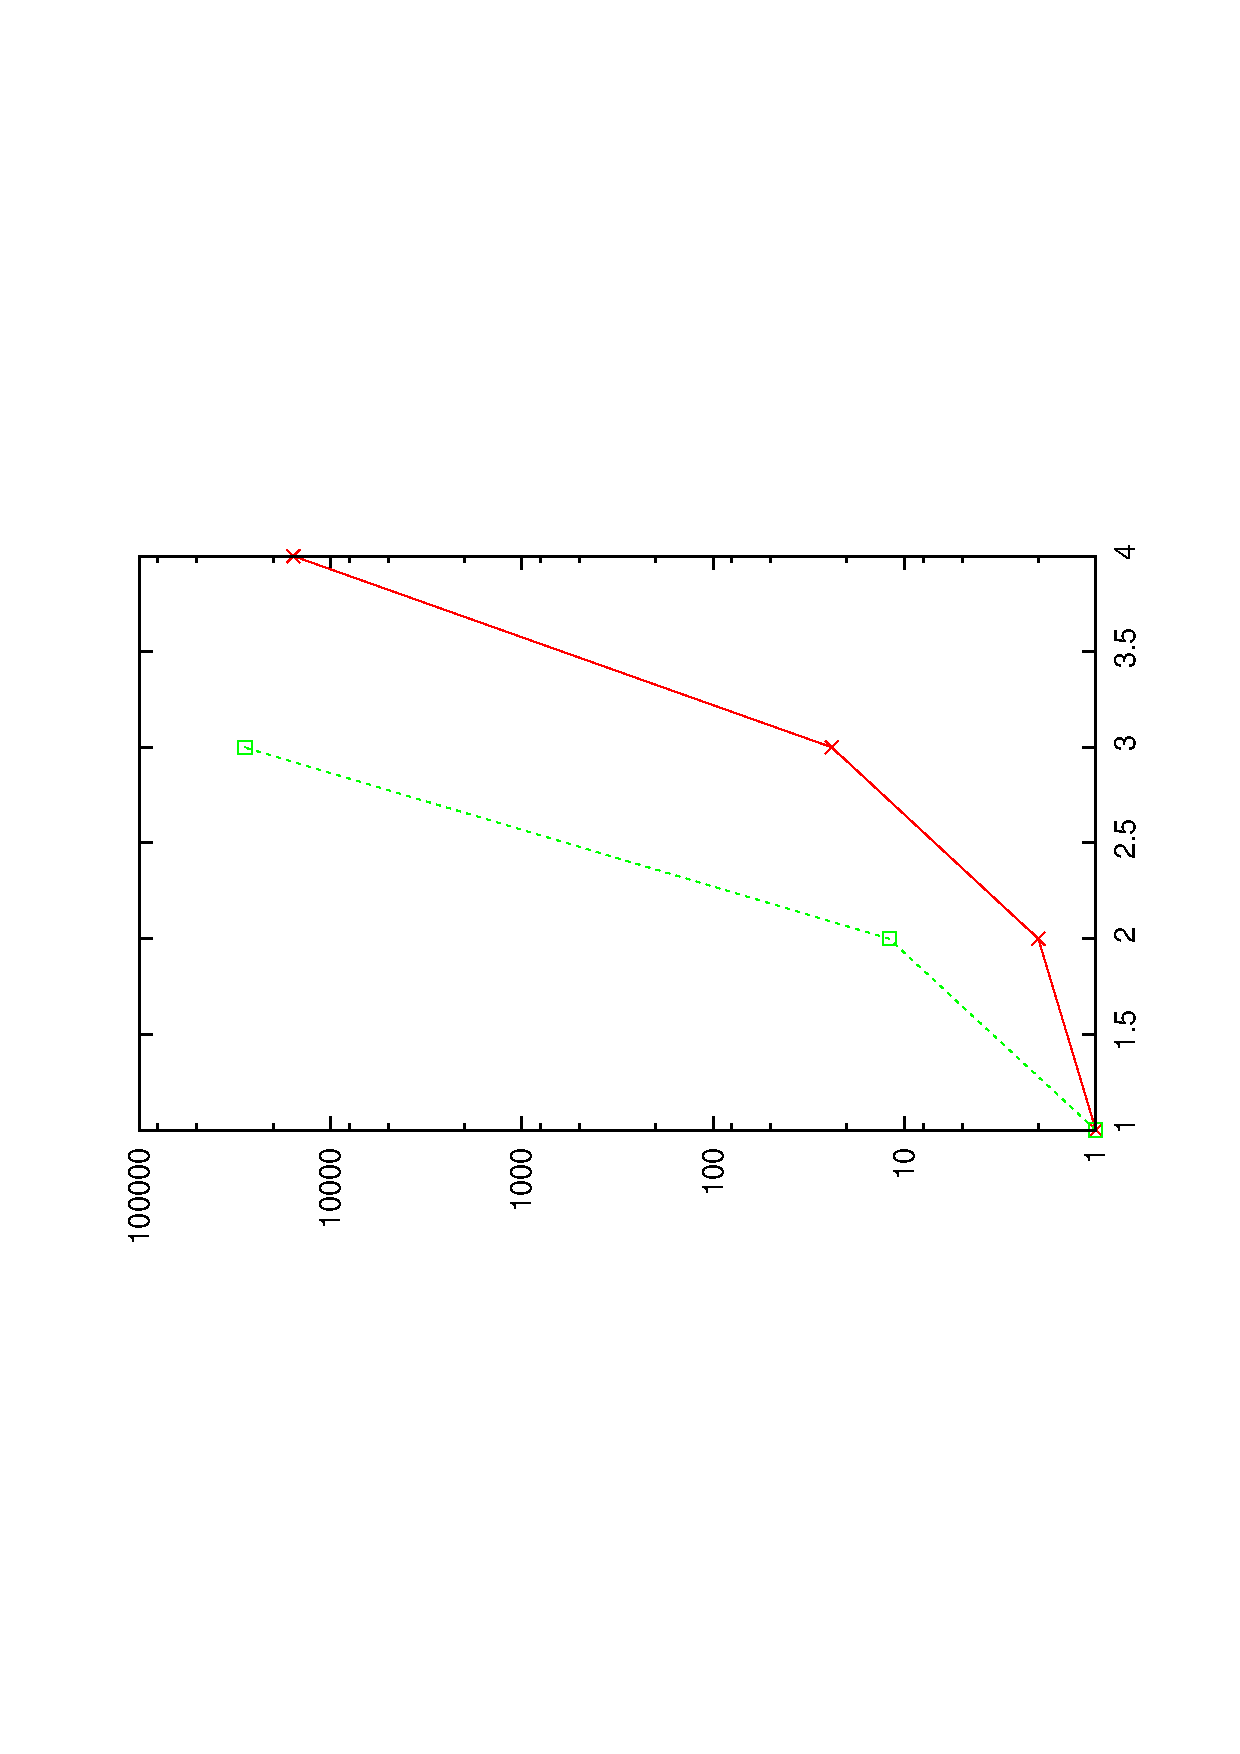
\includegraphics[width=.8\columnwidth]{images/pareto_difference}
		\captionof{figure}{Size of the Pareto-optimal set with (red) and without
		(green) Pareto-optimisation on a logarithmic scale for different
		time-steps}
	   \label{fig:pareto_difference}
	\end{figurehere}
	\vspace{0.5cm}

	Figure \ref{fig:pareto_difference} shows the difference in the set size with
	and without Pareto-optimisation for time-steps up to 4. Although we can see
	that the optimisation reduces the size more than an order of magnitude, it
	also shows that that the size of the set grows faster than exponential in
	both cases.
	The reason for this complexity can be found by analysing the Bellman
	equation (\ref{eq:bellman_q}). The $\max$-operator returns a set of
	solutions for each action, and the sets are summed. As an example to
	illustrate the problem, consider four actions each containing a set of four
	rewards. The result contains each possible sum of any vector from each set.
	This results in a set of $4^4=256$ elements. For the next time-step, this
	would result in a set of $4^{256}\approx 1.34\cdot 10^{154}$ vectors
	(assuming that there were no duplicates and all states had the same set
	size).

	In figure \ref{fig:many_fronts} we can see the distribution of the
	Pareto-fronts per action for several different probabilities with two
	agents. Black represents sending no message, red and green are for the
	different agents, and in the last image the overlapping vectors are shown in
	yellow. Striking is that the points are all located on up to two lines (or
	hyperplanes) per action, where the lines are always perpendicular to the
	line that makes a right angle from the origin. In figure
	\ref{fig:fronts_actions} we can see that the points are also divided in two
	lines per action, which suggests that the number of hyperplanes is
	independent of the time-step, and presumably dependent on the number of
	agents. Figure \ref{fig:t3_555} suggests that this may also hold true for
	more dimensions.
	\end{multicols}

	\begin{figure}
		\centering
		\begin{subfigure}[b]{0.3\textwidth}
			\centering
			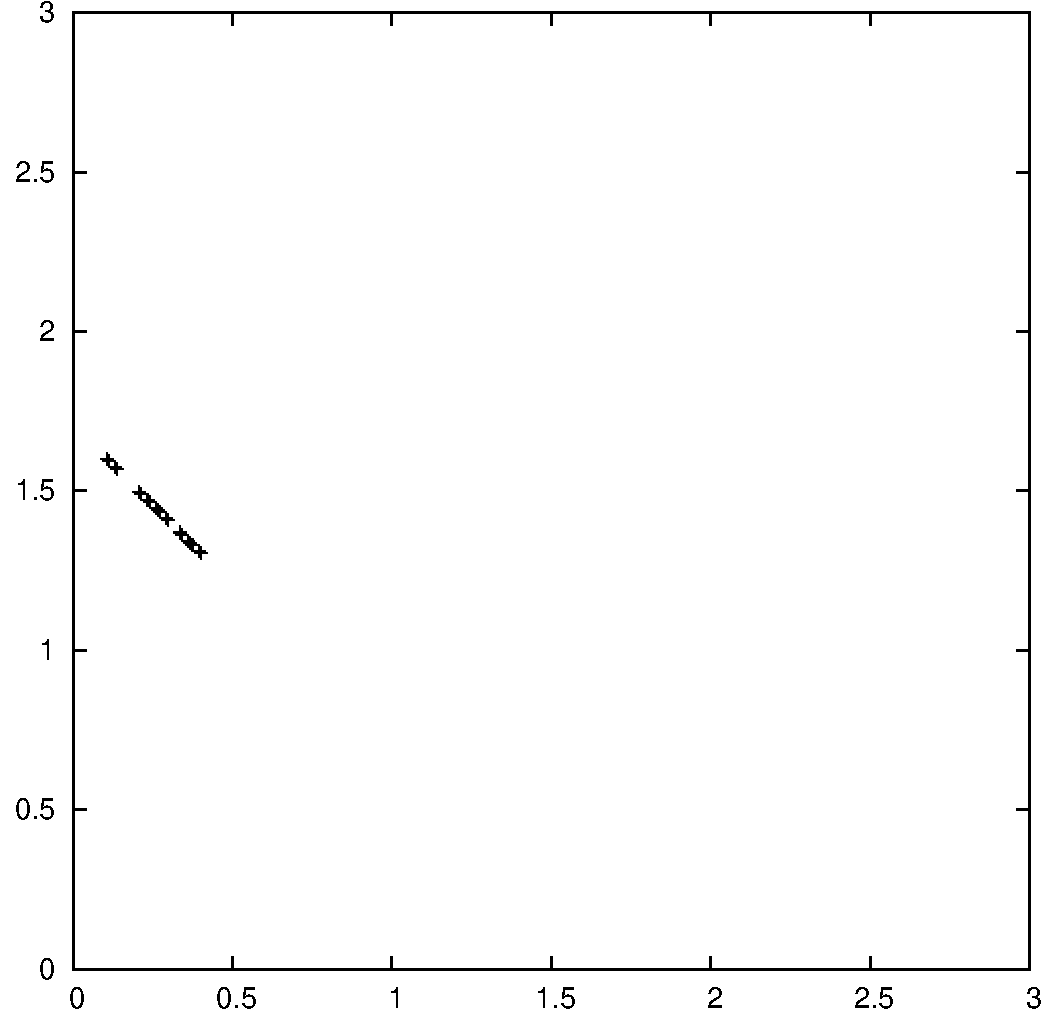
\includegraphics[width=\textwidth]{images/t2s0}
			\caption{$t=2, s=(e,e)$}
			\label{fig:t2s0}
		\end{subfigure}
		~
		\begin{subfigure}[b]{0.3\textwidth}
			\centering
			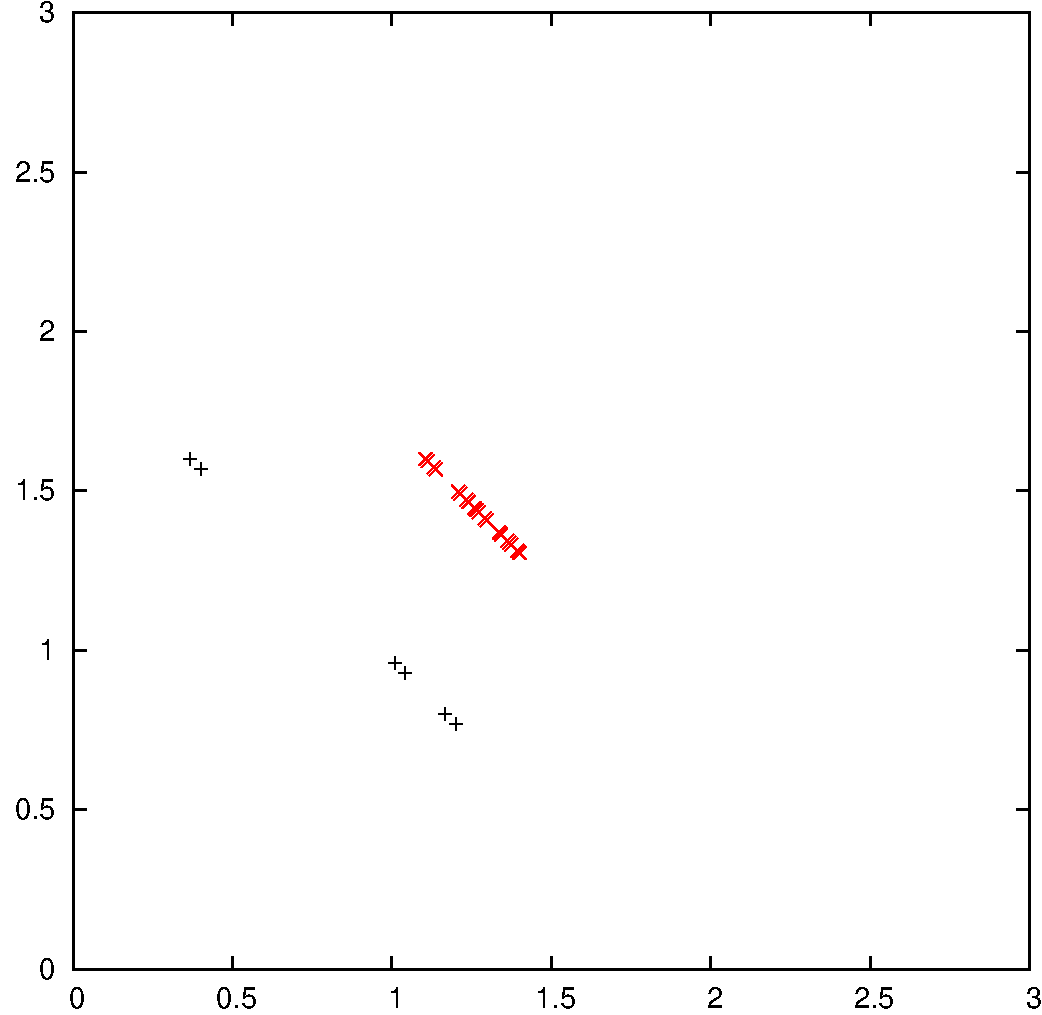
\includegraphics[width=\textwidth]{images/t2s1}
			\caption{$t=2, s=(m,e)$}
			\label{fig:t2s1}
		\end{subfigure}
		~
		\begin{subfigure}[b]{0.3\textwidth}
			\centering
			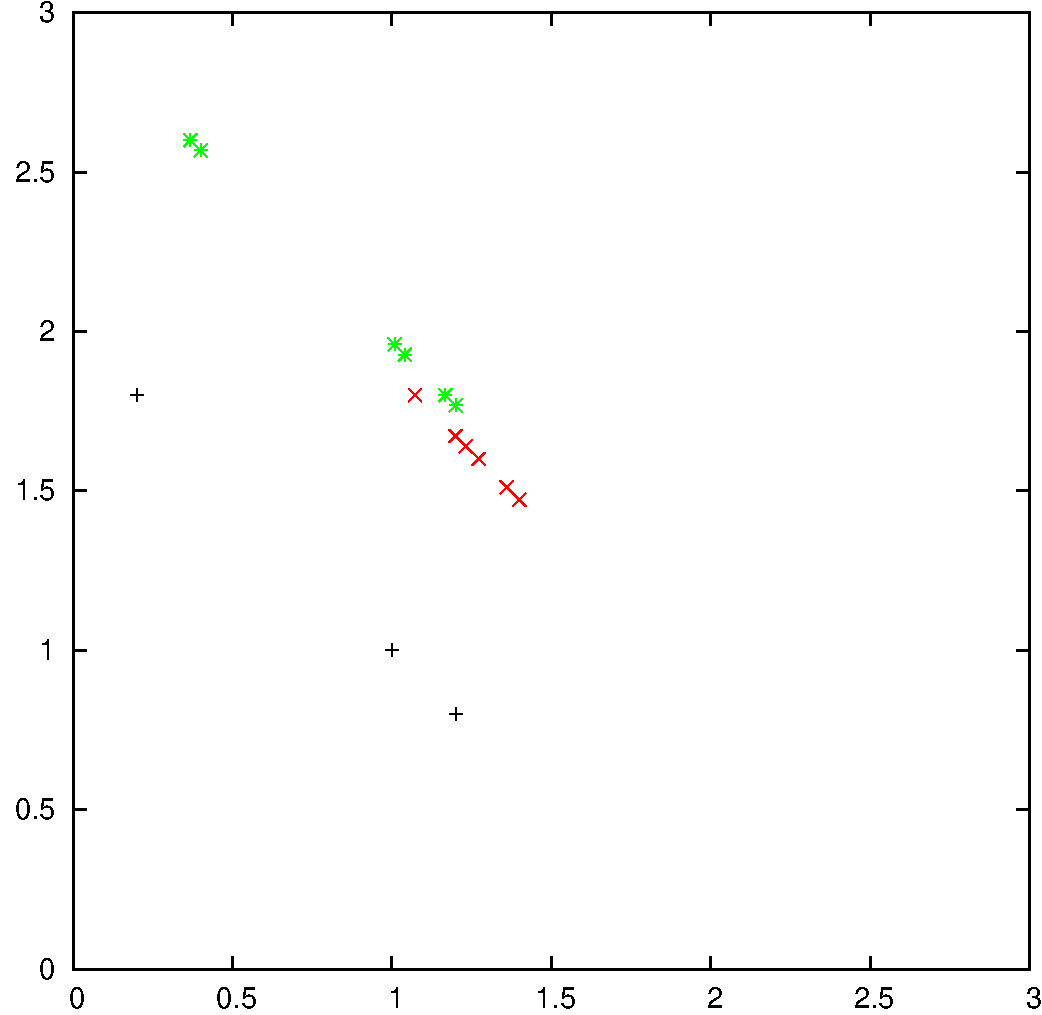
\includegraphics[width=\textwidth]{images/t2s3}
			\caption{$t=2, s=(m,m)$}
			\label{fig:t2s3}
		\end{subfigure}

		\begin{subfigure}[b]{0.3\textwidth}
			\centering
			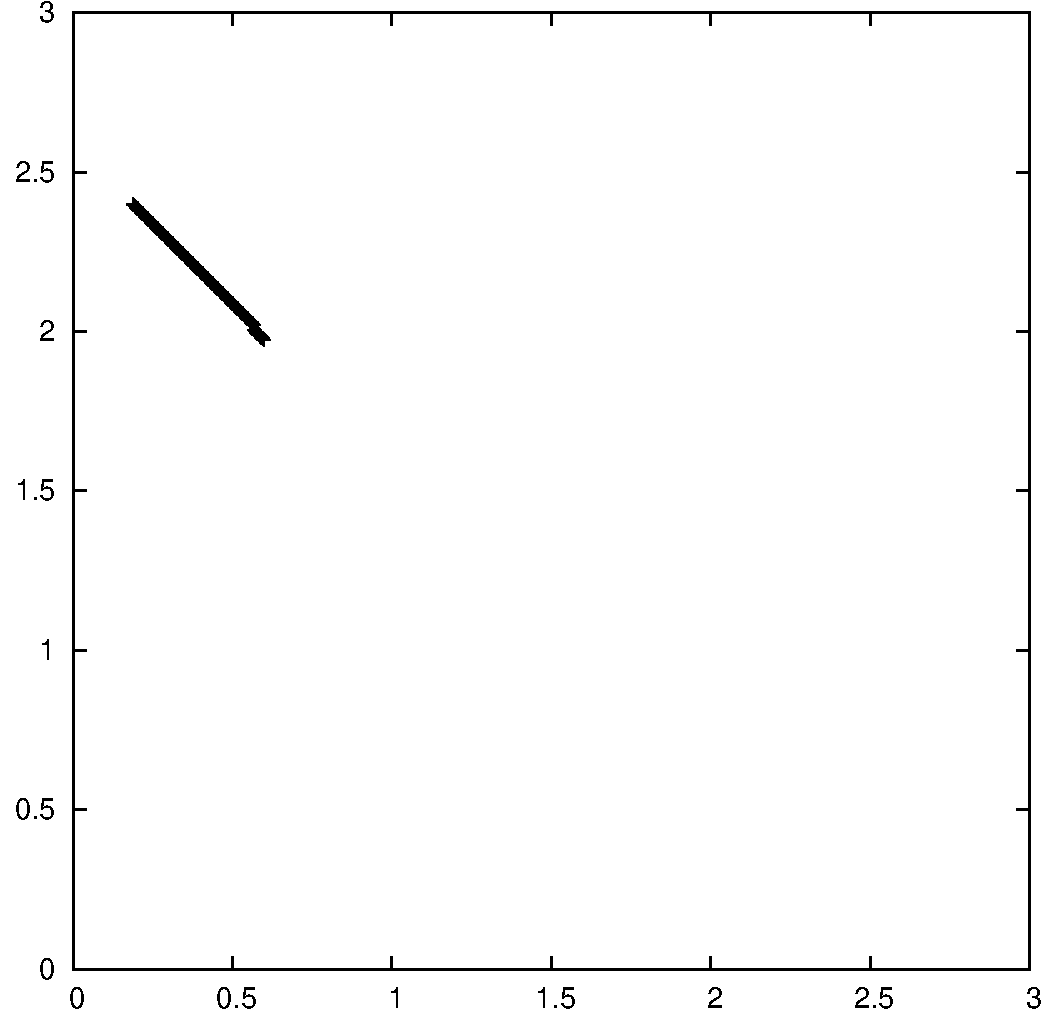
\includegraphics[width=\textwidth]{images/t3s0}
			\caption{$t=3, s=(e,e)$}
			\label{fig:t3s0}
		\end{subfigure}
		~
		\begin{subfigure}[b]{0.3\textwidth}
			\centering
			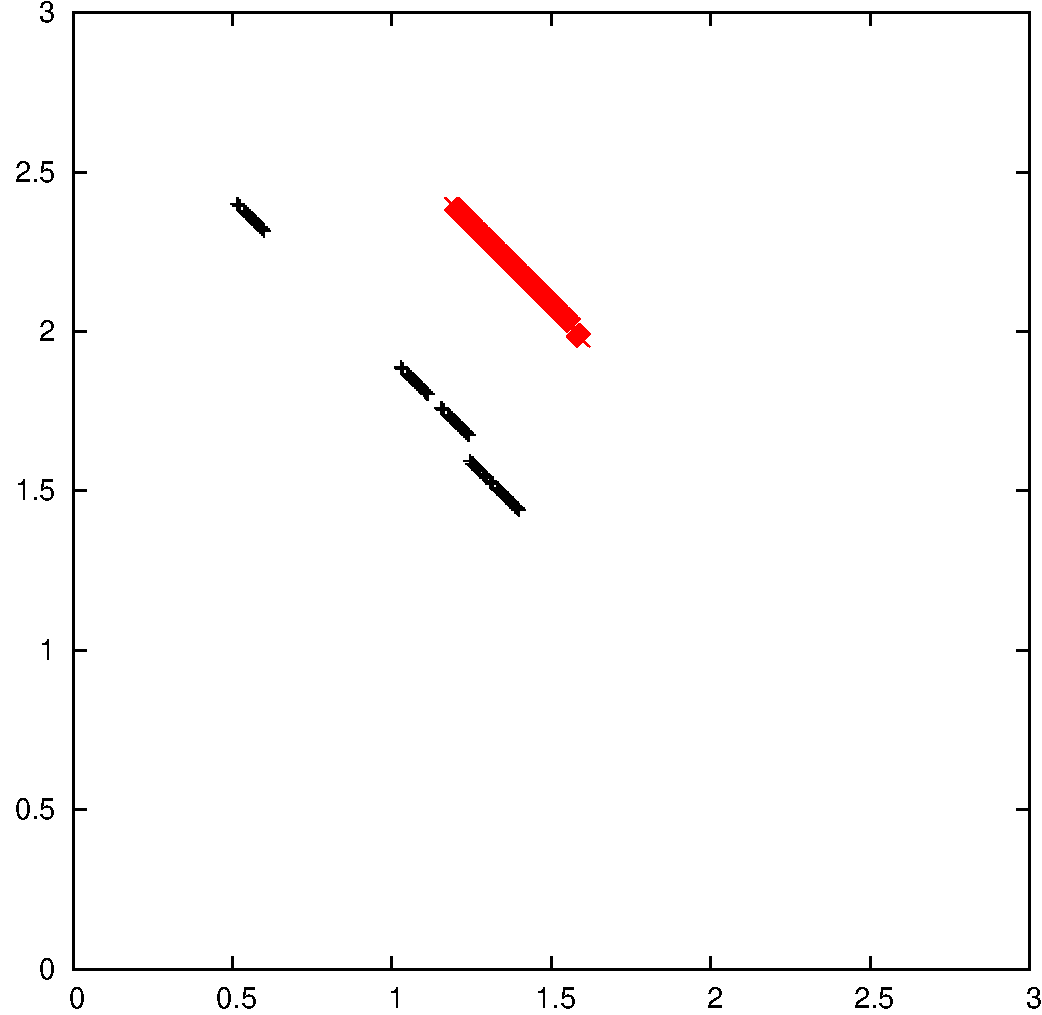
\includegraphics[width=\textwidth]{images/t3s1}
			\caption{$t=3, s=(m,e)$}
			\label{fig:t3s1}
		\end{subfigure}
		~
		\begin{subfigure}[b]{0.3\textwidth}
			\centering
			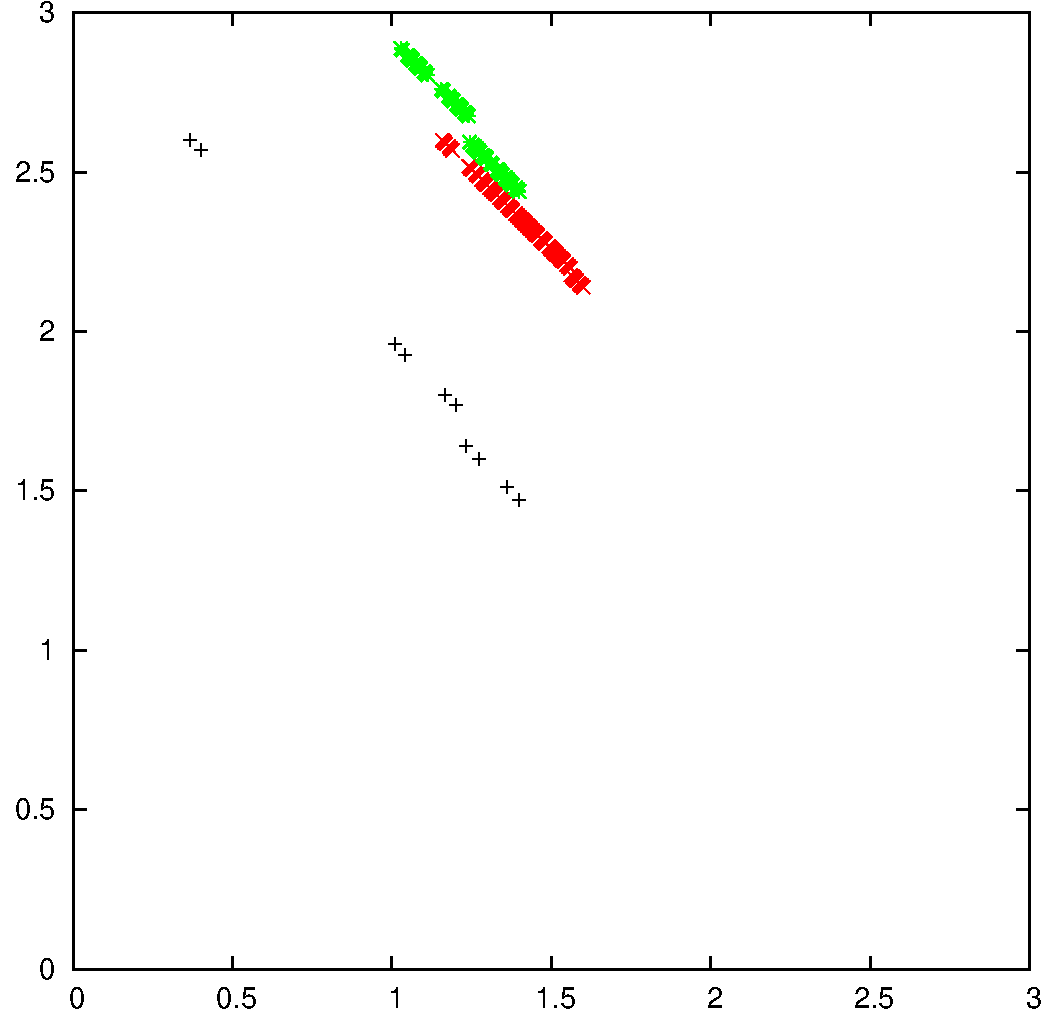
\includegraphics[width=\textwidth]{images/t3s3}
			\caption{$t=3, s=(m,m)$}
			\label{fig:t3s3}
		\end{subfigure}
		\caption{Pareto fronts in time-steps 2 and 3 for different states.
			Colours denote different actions $m$ and $e$ represent a full and an
			empty buffer respectively}
		\label{fig:fronts_actions}
	\end{figure}

	\begin{figure}
		\centering
		\begin{subfigure}[b]{0.45\textwidth}
			\centering
			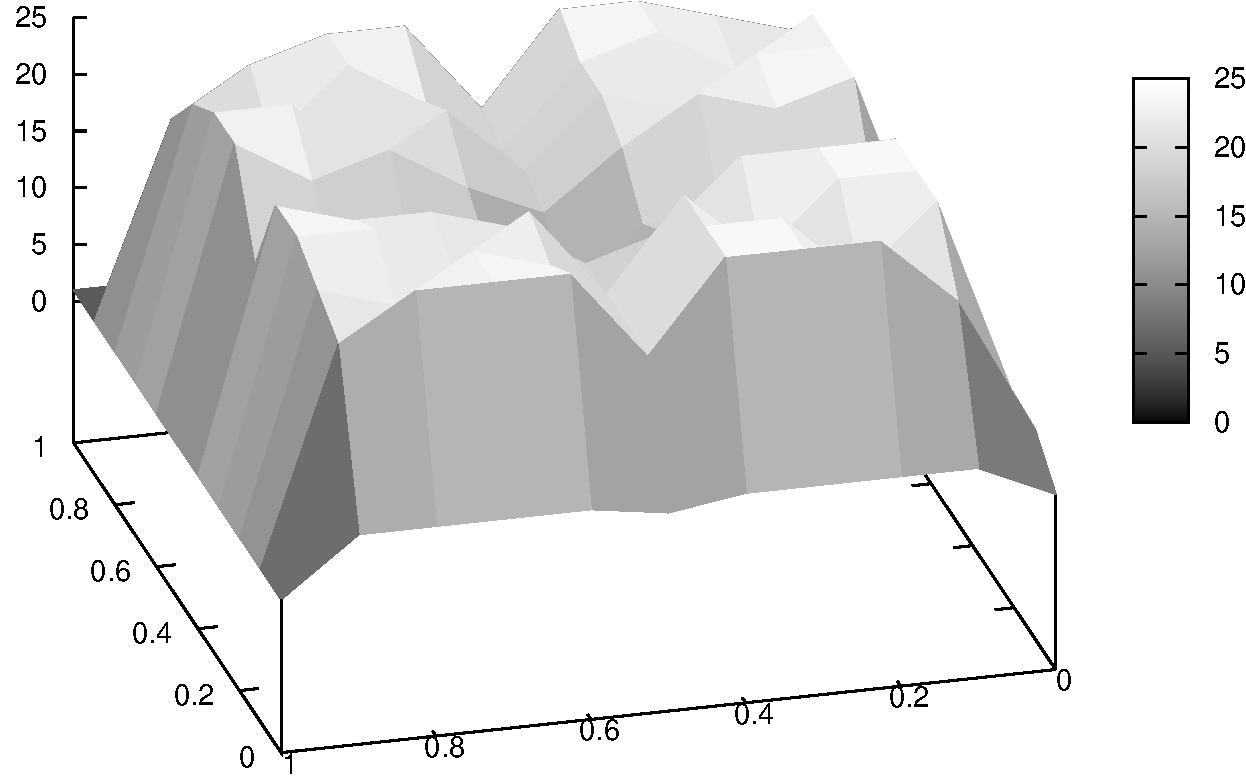
\includegraphics[width=\textwidth]{images/r3_side}
			\caption{$t=3$, From the side}
			\label{fig:r3_side}
		\end{subfigure}
		~
		\begin{subfigure}[b]{0.45\textwidth}
			\centering
			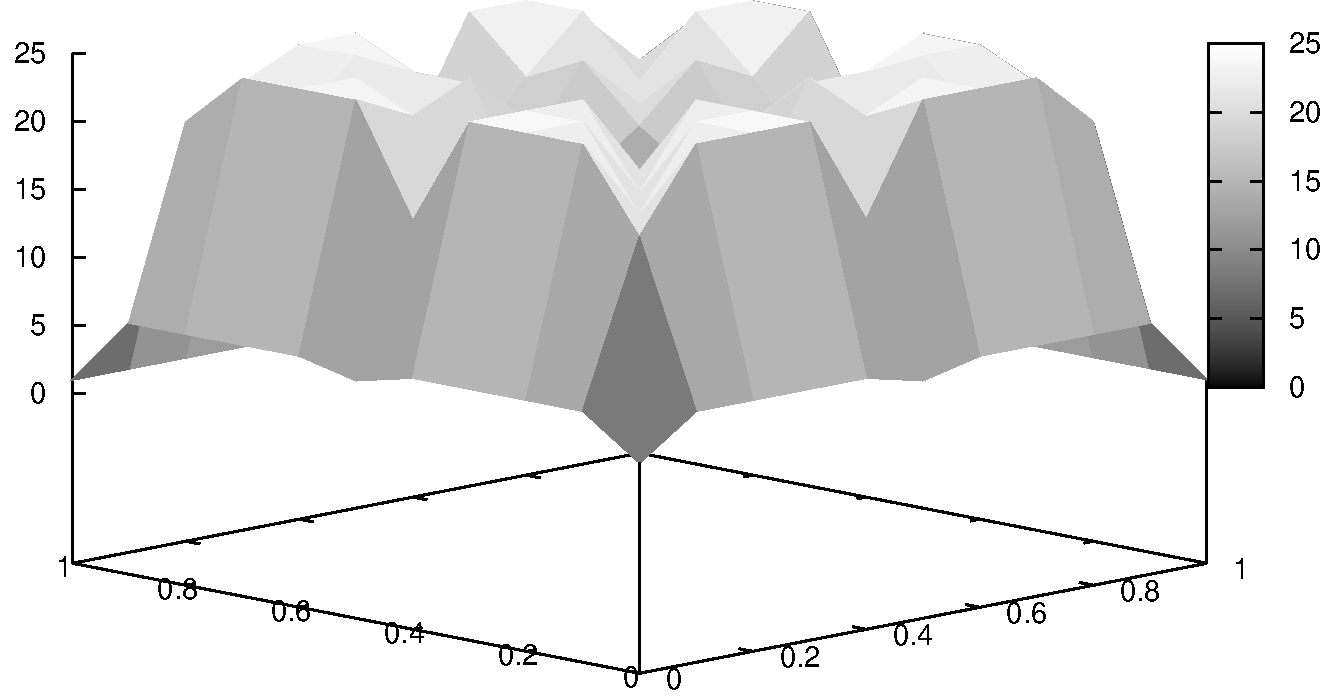
\includegraphics[width=\textwidth]{images/r3_diagonal}
			\caption{$t=3$, Diagonally}
			\label{fig:r3_diagonal}
		\end{subfigure}

		\begin{subfigure}[b]{0.45\textwidth}
			\centering
			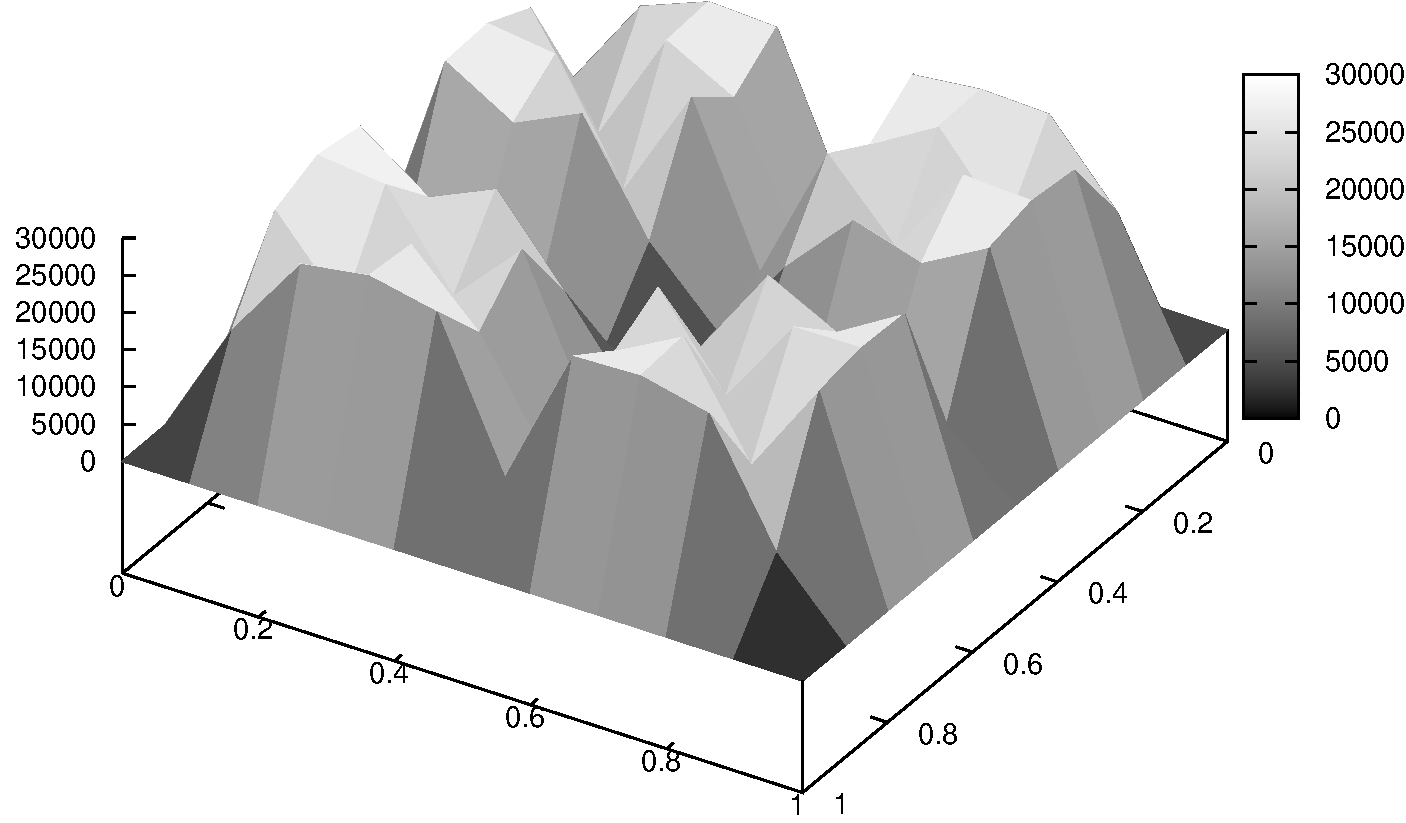
\includegraphics[width=\textwidth]{images/r3_nopareto}
			\caption{$t=3$, Without pareto-optimisation}
			\label{fig:r3_nopareto}
		\end{subfigure}
		~
		\begin{subfigure}[b]{0.45\textwidth}
			\centering
			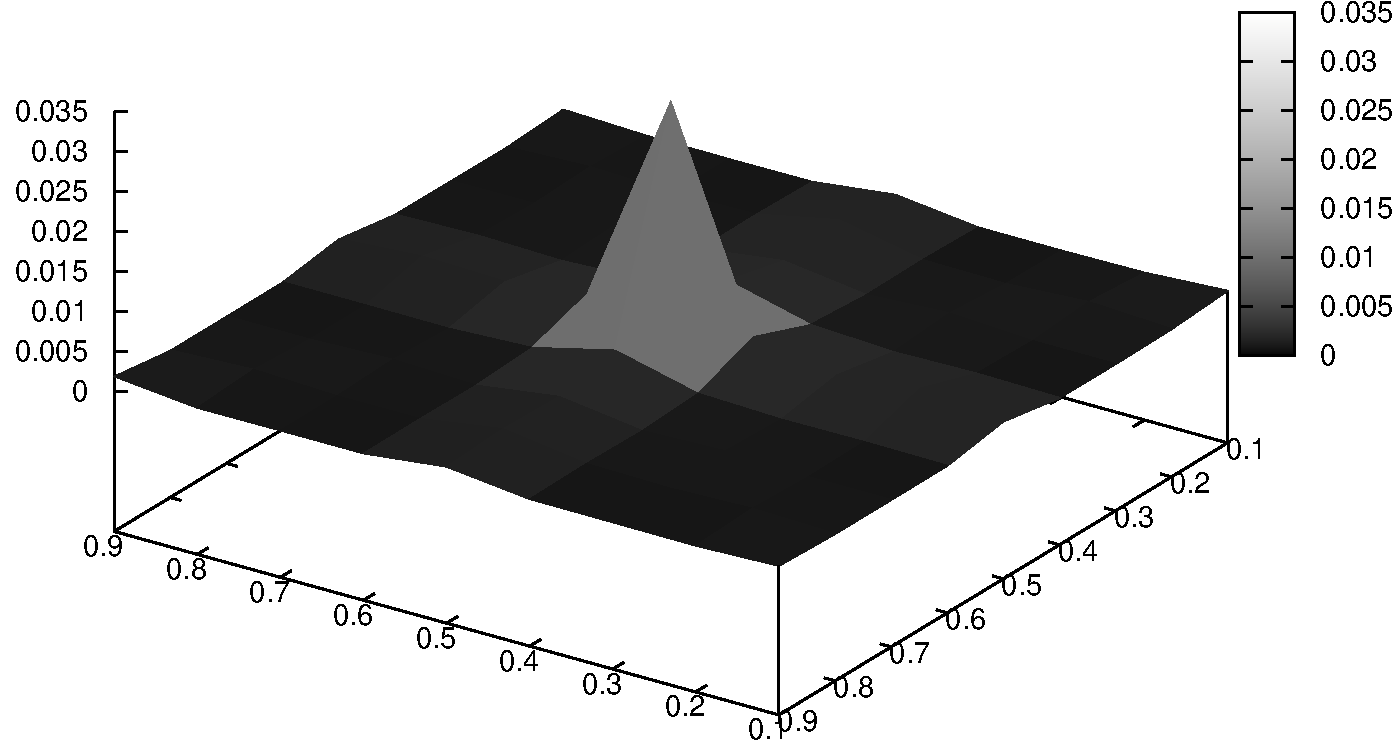
\includegraphics[width=\textwidth]{images/r3_divided}
			\caption{$t=3$, With optimisation / without}
			\label{fig:r3_divided}
		\end{subfigure}

		\centering
		\begin{subfigure}[b]{0.45\textwidth}
			\centering
			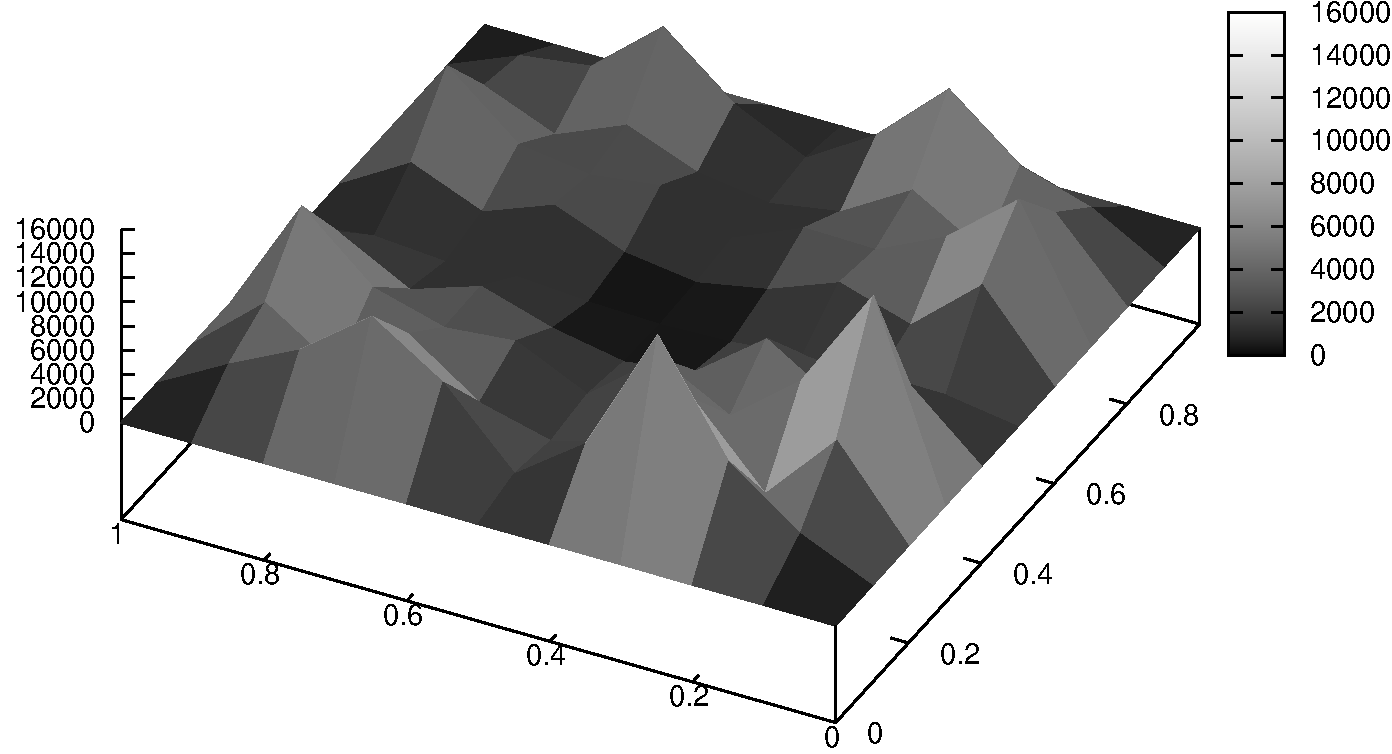
\includegraphics[width=\textwidth]{images/r4_bird}
			\caption{$t=4$, Overview}
			\label{fig:r4_bird}
		\end{subfigure}
		~
		\begin{subfigure}[b]{0.45\textwidth}
			\centering
			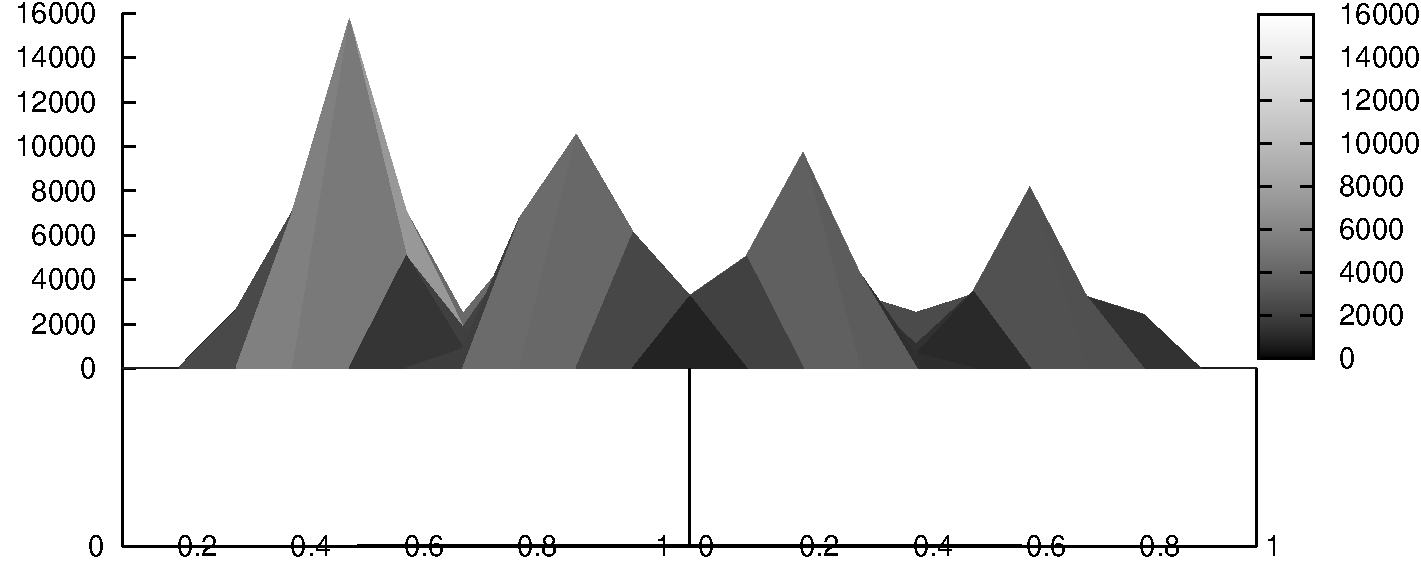
\includegraphics[width=\textwidth]{images/r4_diagonal}
			\caption{$t=4$, Diagonally}
			\label{fig:r4_diagonal}
		\end{subfigure}
		\caption{Size of the pareto-front over different probability
		distributions}
		\label{fig:3d_size}
	\end{figure}

	\begin{figure}
		\centering
		\begin{subfigure}[b]{0.30\textwidth}
			\centering
			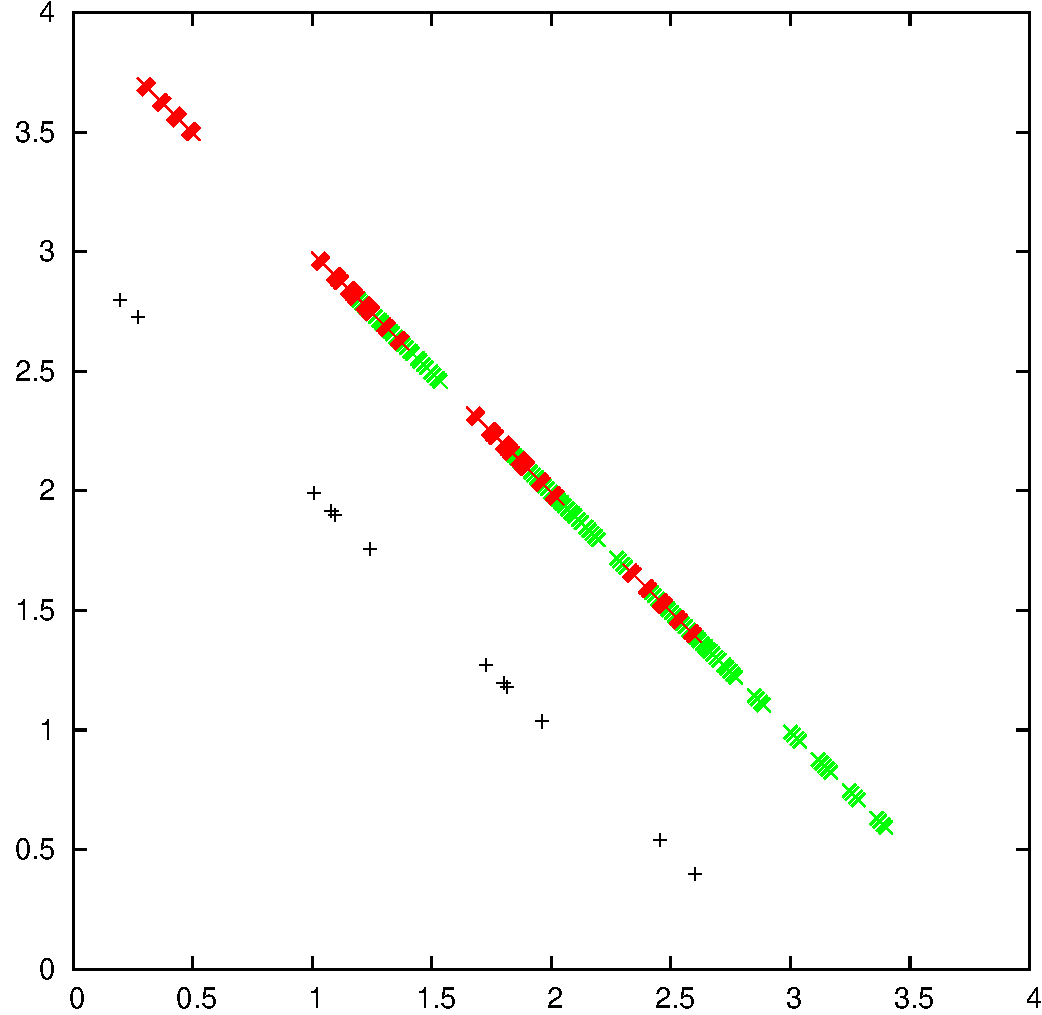
\includegraphics[width=\textwidth,height=7cm,keepaspectratio]{images/t4_12}
			\caption{t=4, p=(0.1, 0.2)}
			\label{fig:t4_12}
		\end{subfigure}
		~
		\begin{subfigure}[b]{0.30\textwidth}
			\centering
			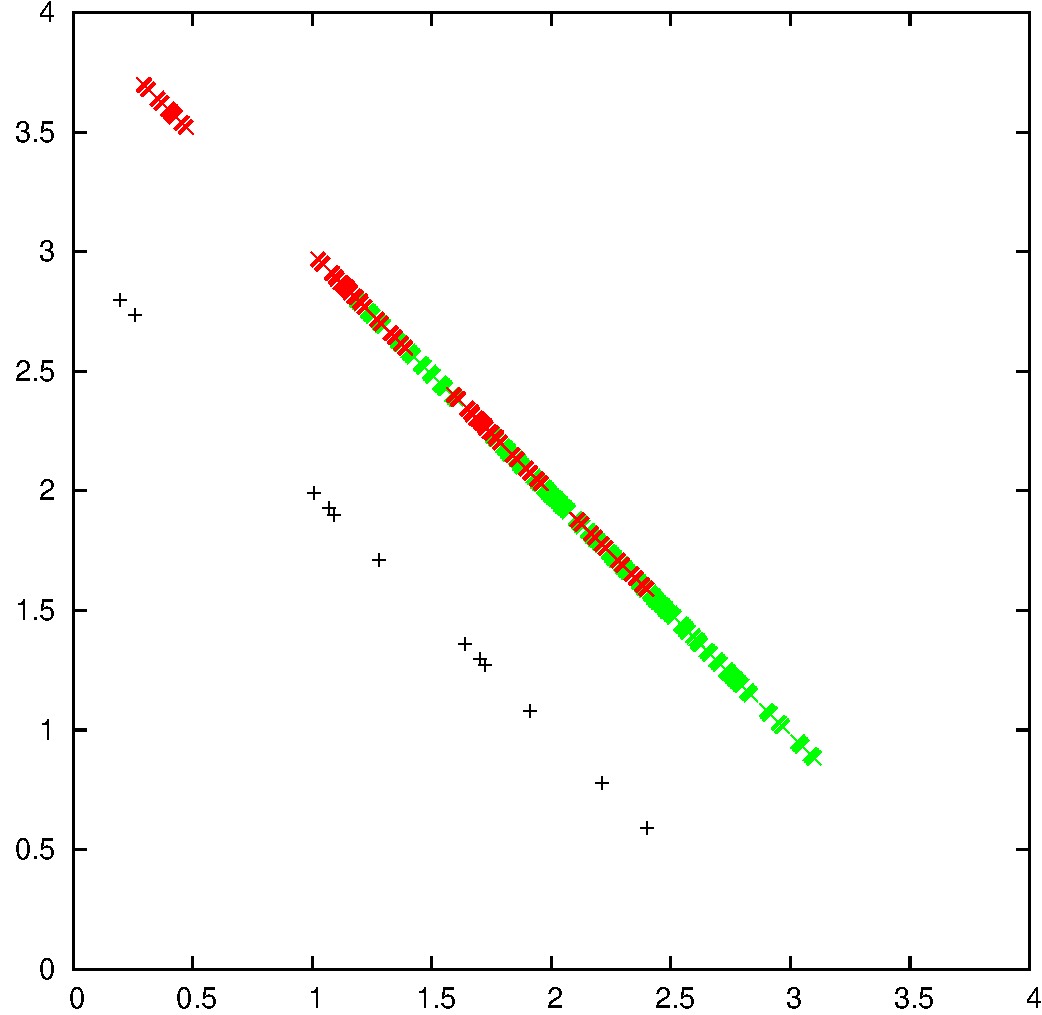
\includegraphics[width=\textwidth,height=7cm,keepaspectratio]{images/t4_13}
			\caption{t=4, p=(0.1, 0.3)}
			\label{fig:t4_13}
		\end{subfigure}
		~
		\begin{subfigure}[b]{0.30\textwidth}
			\centering
			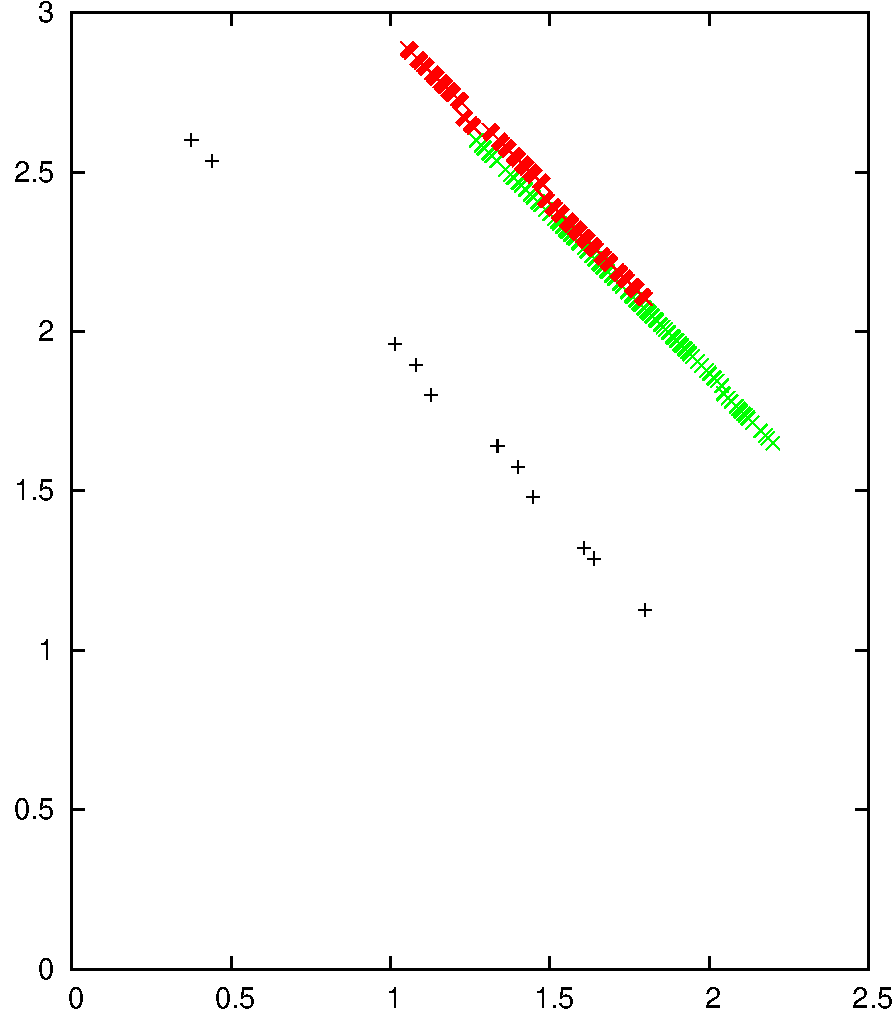
\includegraphics[width=\textwidth,height=7cm,keepaspectratio]{images/t4_26}
			\caption{t=4, p=(0.2, 0.6)}
			\label{fig:t4_26}
		\end{subfigure}

		\begin{subfigure}[b]{0.30\textwidth}
			\centering
			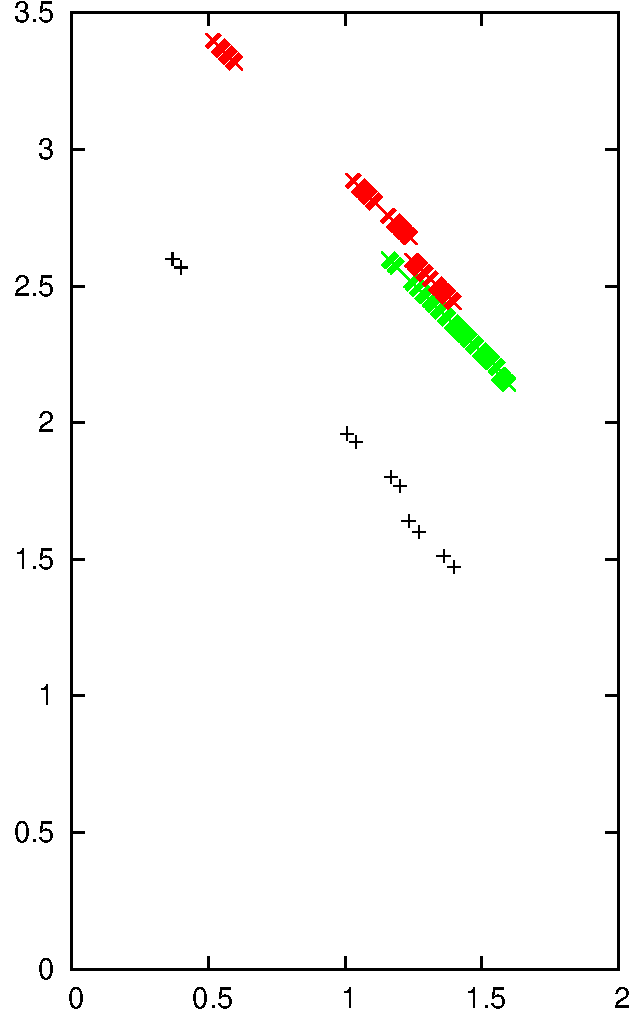
\includegraphics[width=\textwidth,height=7cm,keepaspectratio]{images/t4_28}
			\caption{t=4, p=(0.2, 0.8)}
			\label{fig:t4_28}
		\end{subfigure}
		~
		\begin{subfigure}[b]{0.30\textwidth}
			\centering
			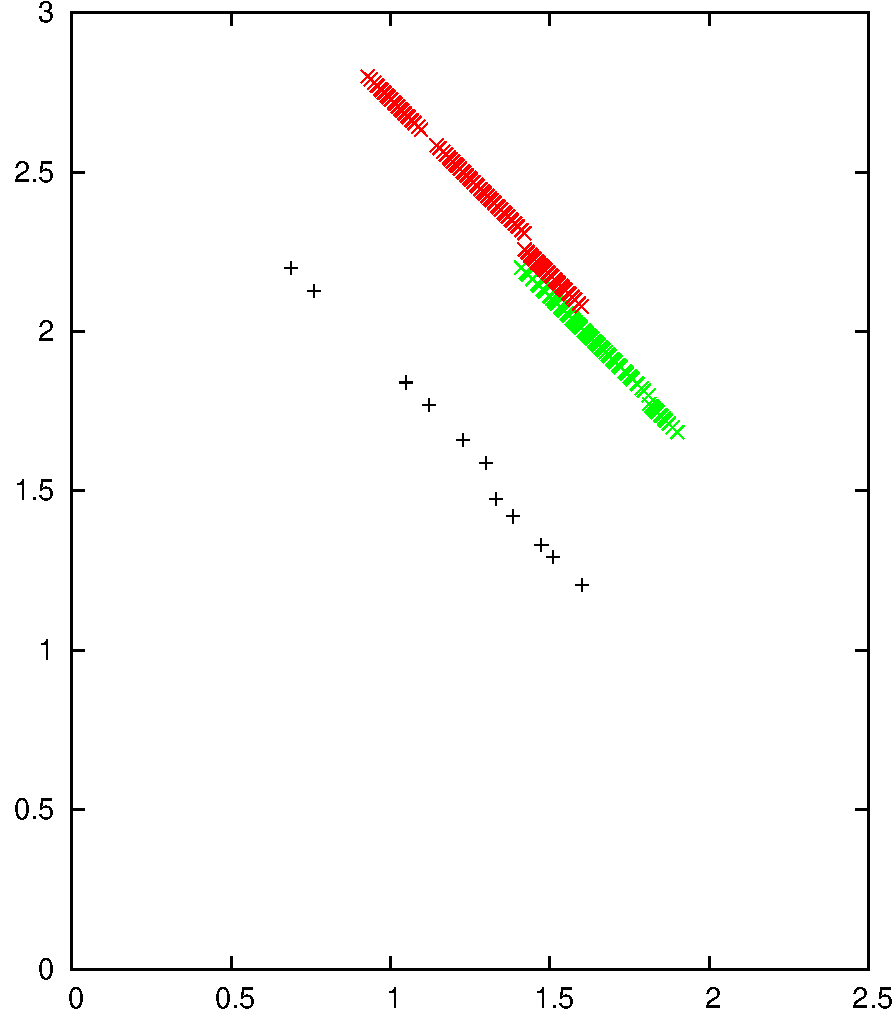
\includegraphics[width=\textwidth,height=7cm,keepaspectratio]{images/t4_47}
			\caption{t=4, p=(0.4, 0.7)}
			\label{fig:t4_47}
		\end{subfigure}
		~
		\begin{subfigure}[b]{0.30\textwidth}
			\centering
			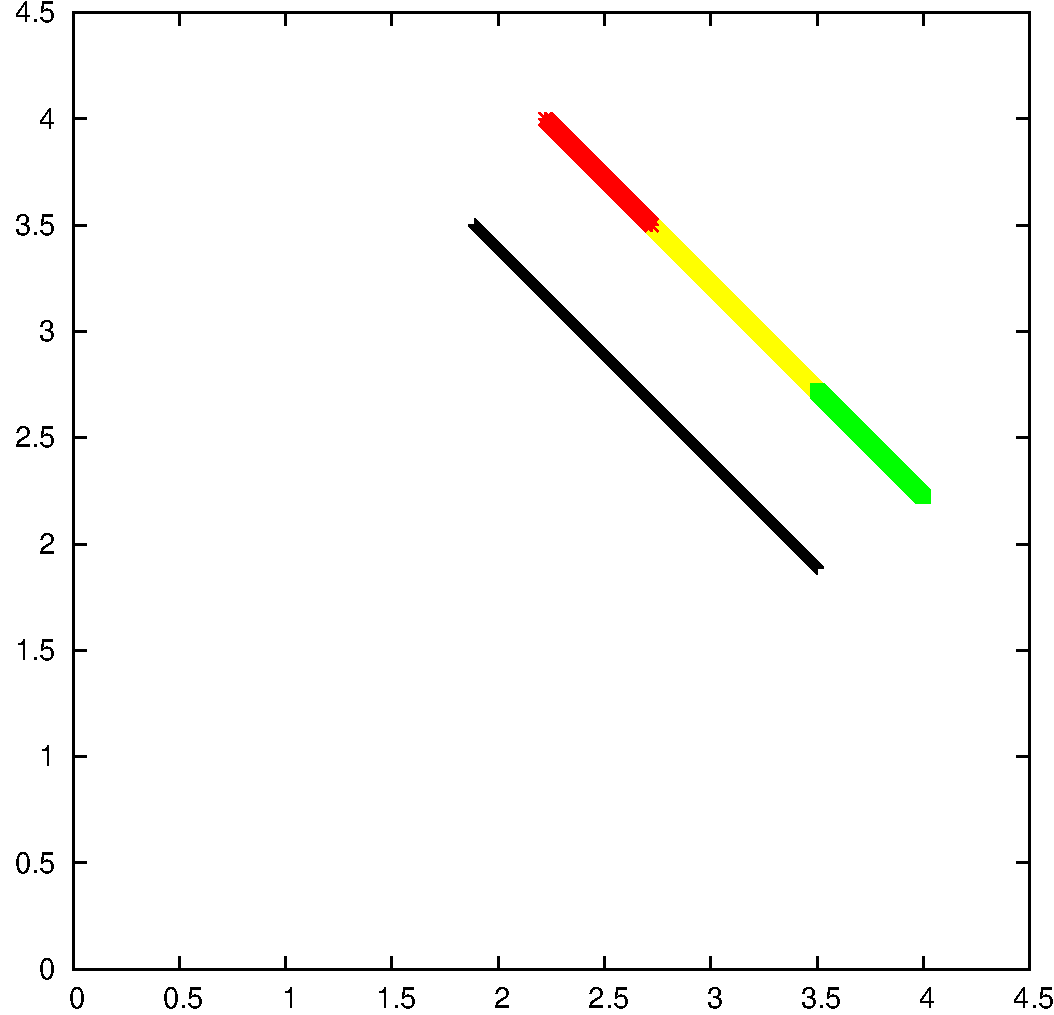
\includegraphics[width=\textwidth,height=7cm,keepaspectratio]{images/t7_55}
			\caption{t=7, p=(0.5, 0.5)}
			\label{fig:t7_55}
		\end{subfigure}
		\caption{Shape of the Pareto-front for different time steps and
			probabilities with two agents. Black indicates no action, green and
			red are for the different actions. Yellow in figure \ref{fig:t7_55} is
			used to show the overlap between values of the two actions. The axes
			represent the throughput of the respective agents}
		\label{fig:many_fronts}
	\end{figure}

	\begin{figure}
		\centering
		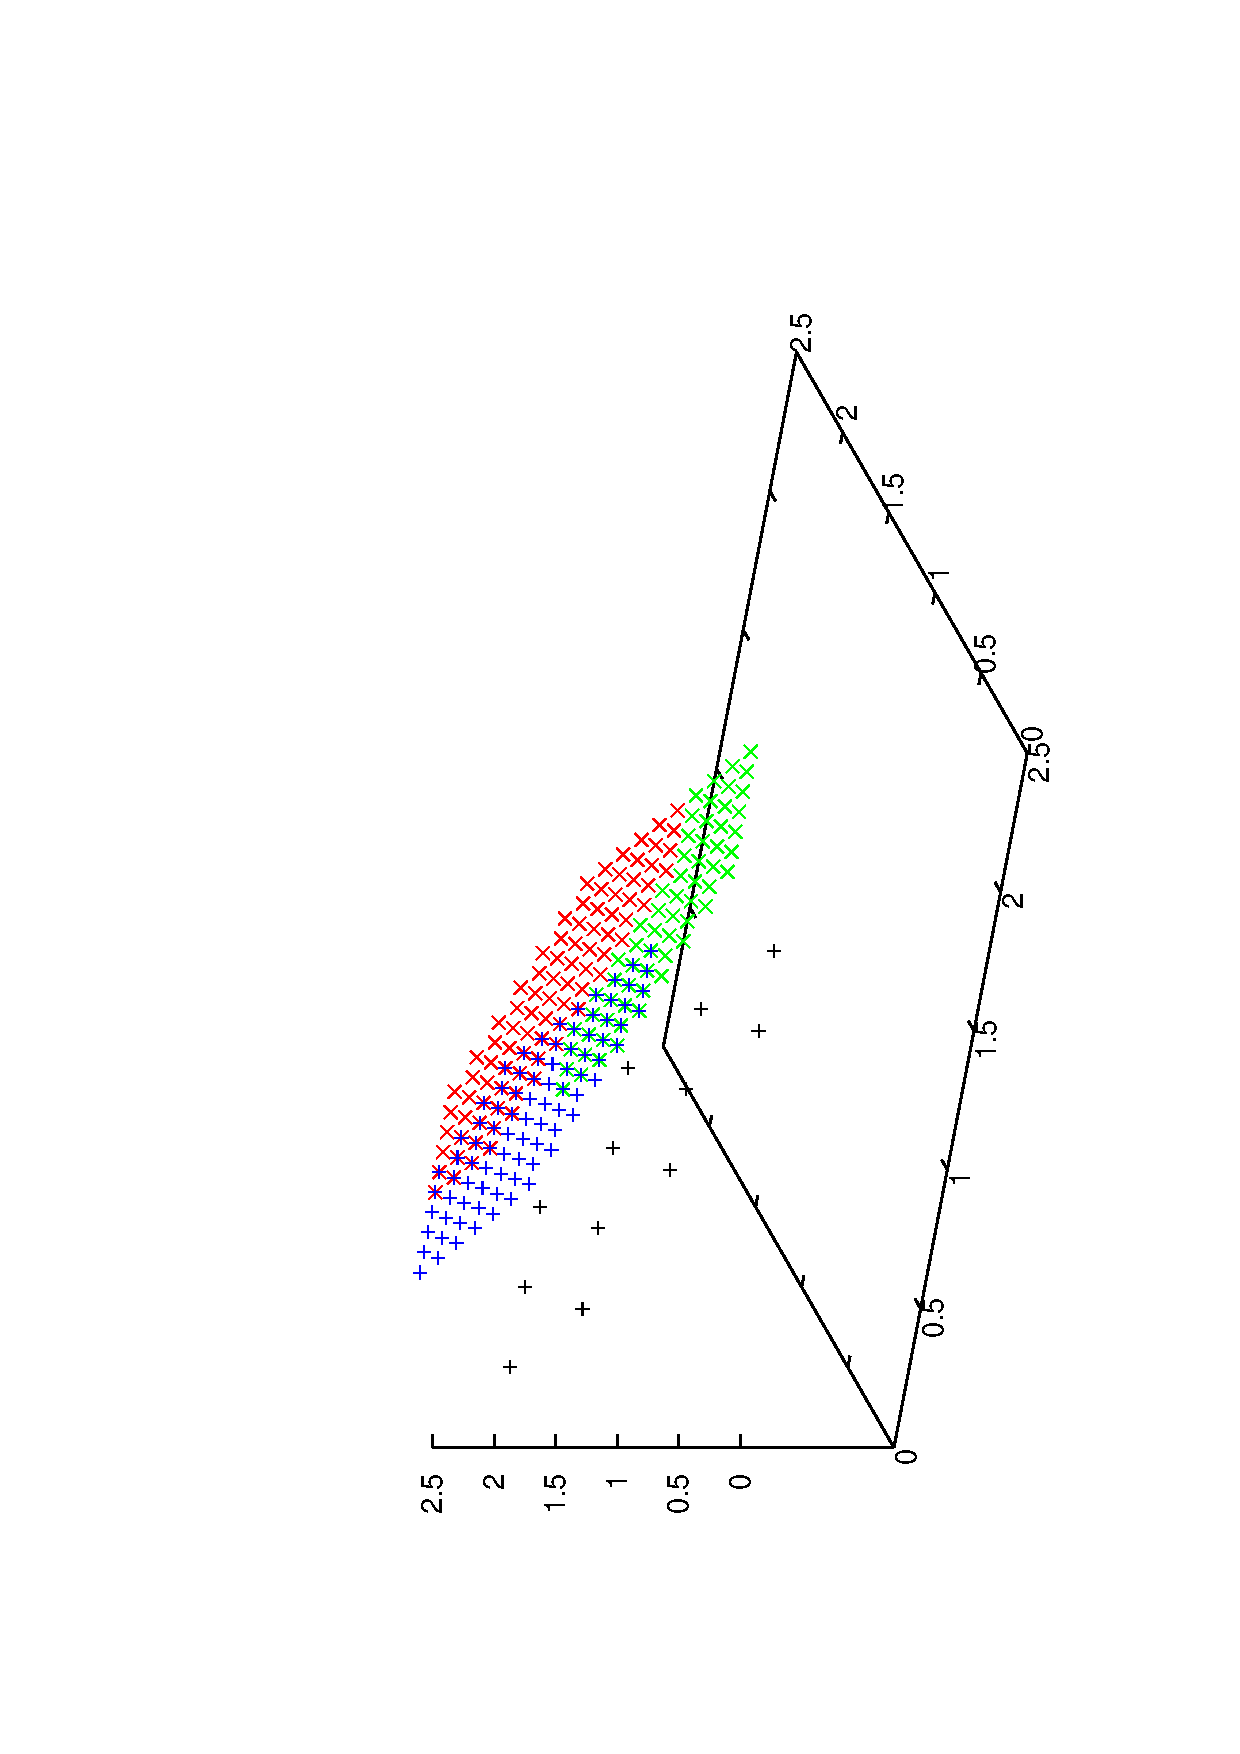
\includegraphics[width=.7\textwidth,height=10cm,keepaspectratio]{images/t3_555}
		\caption{t=3, p=(0.5, 0.5, 0.5)}
		\label{fig:t3_555}
	\end{figure}
	% section results (end)
	%\restoregeometry

	\newpage
	\begin{multicols}{2}
	\section{Discussion}
	\label{sec:discussion}
	Due to computational complexity it was infeasible to calculate the fronts
	for more than two agents, except in the case where all probabilities are
	$0.5$. In future research more aggressive pruning
	(\ref{sub:aggressive_pruning}) could help to analyse the shape of the
	Pareto-set and may confirm or deny our suspicions about the distribution of
	vectors described in section \ref{sec:results}.
	\subsection{Sorted Sets}
		\label{sub:sorted_sets}
		As the C++ implementation of the \texttt{set} class is sorted, it is
		possible to select subsets based on separators. In the case of adding a
		new vector to the set there are three distinct possible situations:
		\begin{enumerate}
			\item Elements must be removed and the new vector added
			\item No elements must be removed but the new vector must be added
			\item No elements must be removed and the new vector must not be added
		\end{enumerate}
		When we consider the whole set per dimension, we can separate the vectors
		in the set into three different sets of interest:
		\begin{enumerate}
			\item Elements that may be strictly better
			\item Elements that may be strictly worse
			\item Elements that are not better or worse
		\end{enumerate}
		Sets 1 and 2 may intersect when the values of the vector that have been
		compared are the same as the vector that is to be added.  The fist and
		second categories contain values that are equal or larger or equal or
		smaller in each evaluated dimension respectively. Vectors that have a
		higher value in at least one dimension and a lower value in another, fall
		in the third category. All vectors that have been identified as belonging
		in the third category can be excluded from evaluation, as they do not
		affect the actions that must be performed. As we explore more dimensions
		the size of the third set will increase and the first two will decrease.

		When we have reached the last dimension, the sets tell us what action to
		take:
		\begin{itemize}
			\item If set 1 is not empty: do not add (situation 3)
			\item Else if set 2 is not empty: remove all vectors from this set and
				add the new vector (situation 1),
			\item Else (sets 1 and 2 are empty): add the new vector (situation 2).
		\end{itemize}

		Since the sets are in a large part distributed on a few lines, as can be
		seen in figures \ref{fig:fronts_actions}, and \ref{fig:many_fronts}, we
		could represent them as several sets, grouped by the lines they are on.
		As all points are on a single line, the vectors in the set are sorted in
		both the first and the second dimension.

		All points of interest for ruling out that the vector are in the quadrant
		that contains only vectors that are higher or equal to the new vectors in
		the first two dimensions. By using these features we can reduce the
		amount of vectors that need to be compared to about a quarter.

	\vspace{0.5cm}
	\begin{tablehere}
		\centering
		\begin{tabular}{|lll|}
		\hline
		0		&	0.1	&	1.9\\
		0		&	1		&	1\\
		0		&	1.7	&	0.3\\
		\hline
		0.1	&	0		&	1.9\\
		0.1	&	0.9	&	1\\
		\hline
		0.3	&	1		&	0.7\\
		0.3	&	1.7	&	0\\
		\hline
		0.7	&	1		&	0.3\\
		\hline
		0.9	&	0.1	&	1\\
		\hline
		1		&	0		&	1\\
		1		&	0.2	&	0.8\\
		1		&	0.8	&	0.2\\
		1		&	1		&	0\\
		\hline
		1.2	&	0		&	0.8\\
		1.2	&	0.8	&	0\\
		\hline
		\end{tabular}
		\captionof{table}{Example Front: $s=(e,e)$, $p=(.1 .3 .8)$, $t=2$}
		\label{tab:t2_138}
	\end{tablehere}
	% subsection sorted_sets (end)

	\subsection{Aggressive Pruning}
		\label{sub:aggressive_pruning}
		Figure \ref{fig:pareto_difference} shows that the complexity of the
		algorithm is worse than exponential, and therefore it is not usable
		beyond around four time-steps in a set-up with two agents, and fewer
		time-steps for more agents. This makes it necessary to prune the set, for
		example by using only the $\varepsilon$-approximate Pareto-set.
		Clustering algorithms could be used to keep the set on a constant maximum
		size for any time-step.
	% subsection aggressive_pruning (end)
	% section discussion (end)
	\end{multicols}

	\clearpage
	\bibliographystyle{plainnat}
	\bibliography{references}
\end{document}

% Notes
% FIXME: Only works on last two dimensions, only one dimension at the
% time
%
% 1	.9		.4
% 1	.8		.5
% 1	.7		.6
% 1	.6		.7
% 1	.5		.8
% 1	.4		.9
%					<- last two dimensions are sorted; can be categorised in
%						one go when the first n-2 values are the same
% 1.1	.8		.5
% 1.1	.7		.6
% 1.1	.6		.7
% 1.1	.5		.8
% may work if we save all vectors together that start with the same
% values
%
% Should be a tree for the first n-2 dimensions. C++: multimap
%
% 0.0	-> 0.0 -> [...]
%		-> 0.5 -> [...]
%		-> 1.0 -> [...]
%		-> 1.5 -> [...]
%
% 0.5	-> 0.0 -> [...]
%		-> 0.5 -> [...]
%		-> 1.0 -> [...]
%		-> 1.5 -> [...]
%
% 1.0	-> 0.0 -> [...]
%		-> 0.5 -> [...]
%		-> 1.0 -> [...]
%
% 1.5	-> 0.0 -> [...]
%		-> 0.5 -> [...]
%
% (n-2 * for (1/2 n))
% (1/2)^(n-2)*2*log(n)
%
% discovering in which line(/hyperplane) a vector is (for adding):
% unique key of hyperplane: norm of orthogonal projection on [1 1 1 1 1 ...]
% = abs(dot(v, n/|n|)) met n = [1 1 1 1]'/norm (with error margin)

